\section{Gestion des TDs}

\begin{center}
\scalebox{0.7}{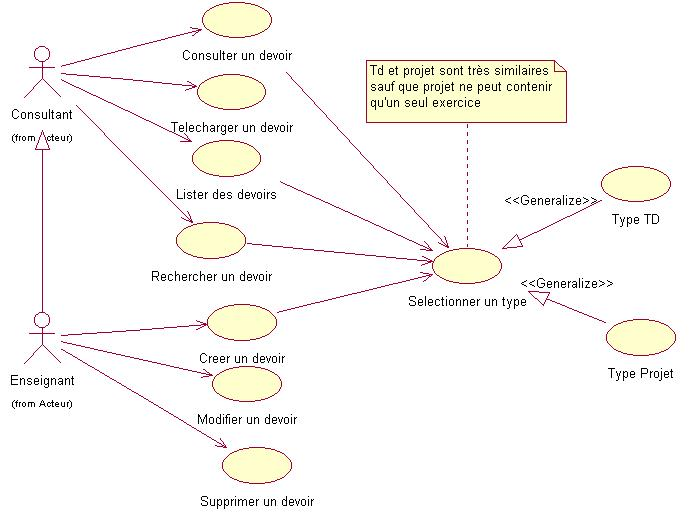
\includegraphics{images/devoir.jpg}}\\
\end{center}

\section*{Consultant}
\begin{tabular}{|p{4cm}|c|p{4cm}|p{5cm}|}
\hline
Fonction & Priorit{\'e} & Qualit{\'e} & Mesure \\
\hline
Rechercher un TD & 4 & rapide et pr{\'e}cis & La recherche doit {\^e}tre efficace.\\
\hline
Consulter un TD & 5 & rapide et clair & la lisibilit{\'e} de projet doit {\^e}tre facile et agr{\'e}able {\`a} lire.\\
\hline
T{\'e}l{\'e}charger un TD & 2 & fiable et rapide & Le temps de t{\'e}l{\'e}chargement ne doit pas {\^e}tre {\'e}lev{\'e}.\\
\hline
\end{tabular}

\begin{center}
{\'e}chelle de mesure de la priorit{\'e}:

\scalebox{0.5}{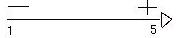
\includegraphics{images/echelle.jpg}}
\end{center}

\begin{itemize}
\item {\bf Rechercher un TD :}
	\begin{itemize}
	\item Pr{\'e}-requis : Il faut qu'il y ait au moins un TD de cr{\'e}{\'e}.
	\item Description : Il saisie les mots clefs de sa recherche s'il en a dans la case {\it Mots clefs}.
	Il valide l'option {\it Recherche}.
	Une liste de TD apparait.
	\item Post-requis : La saisie de mot clefs est optionnel, Si aucun mot clefs n'est saisie, la recherche liste l'ensemble des TDs.\\
	La liste de TD trouv{\'e}s peut contenir de zero {\`a} plusieurs TDs.\\
	\end{itemize}
\item {\bf Consulter un TD :}
	\begin{itemize}
	\item Pr{\'e}-requis :Il faut qu'il y ait au moins un TD de cr{\'e}{\'e}.
	\item Description : Il s{\'e}lectionne successivement les liens lui permettant d'atteindre un TD (ou par recherche).\\
	Il clique pour le visualiser.
	\item Post-requis : Le TD s{\'e}lectionn{\'e} est affich{\'e} au format HTML.\\
	\end{itemize}
	
\item {\bf T{\'e}l{\'e}charger un TD :}
	\begin{itemize}
	\item Pr{\'e}-requis :Il faut qu'il y ait au moins un devoir de cr{\'e}{\'e} et que l'utilisateur ait s{\'e}lectionn{\'e} un TD.
	\item Description : L'utilisateur clique l'option {\it T{\'e}l{\'e}charger}, il s{\'e}lectionne l'emplacement sur son compte pour copier le devoir et valide.
	\item Post-requis : Le TD est copi{\'e} sur le compte du consultant.\\
	\end{itemize}
\end{itemize}

\section*{Responsable}
\begin{tabular}{|p{4cm}|c|p{4cm}|p{5cm}|}
\hline
Fonction & Priorit{\'e} & Qualit{\'e} & Mesure \\
\hline
Cr{\'e}er un TD & 5 & facile & Doit {\^e}tre facile d'utilisation.\\
\hline
D{\'e}placer vers la corbeille & 2 & fiable & il ne doit pas y avoir de perte d'information.\\
\hline
\end{tabular}

\begin{center}
{\'e}chelle de mesure de la priorit{\'e}:

\scalebox{0.5}{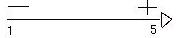
\includegraphics{images/echelle.jpg}}
\end{center}

\begin{itemize}
\item {\bf Cr{\'e}er un TD :}
	\begin{itemize}
	\item Pr{\'e}-requis : Etre identifi{\'e}.
	\item Description : Il s'identifie avec son login et son mot de passe.\\
	Il s{\'e}lectionne le lien lui permettant de se diriger vers la page de cr{\'e}ation du devoir.\\
	Il s{\'e}lectionne l'enseignement pour lequel le devoir est destin{\'e}.\\
	Il choisit s'il cr{\'e}e compl{\'e}tement un nouveau TD ou s'il se sert d'un ancien TD :
	\begin{itemize}
		\item : S'il cr{\'e}e un nouveau TD : Il saisie les mots clefs qui serviront pour la recherche de ce TD.\\
		Il s{\'e}lectionne un ou plusieurs exercices dans une liste d'exercices pr{\'e}-enregistr{\'e}s ou il le(s) importe.\\
		Il choisit la hi{\'e}rarchie des exercices contenus dans son TD.
		\item : S'il se sert d'un ancien TD : Le nouveau TD est une copie de l'ancien et l'utilisateur peut alors le modifier.
	\end{itemize}
	Il valide sa s{\'e}lection.
	\item Post-requis : Un nouveau TD est enregistr{\'e} dans la liste des TD disponibles.\\
	\end{itemize}

\item {\bf D{\'e}placer vers la corbeille :}
	\begin{itemize}
	\item Pr{\'e}-requis : Etre identifi{\'e}.\\
	Il faut qu'au moins un TD soit enregistr{\'e}.\\
	Il doit {\^e}tre le cr{\'e}ateur du TD.
	\item Description : Il s'identifie avec son login et son mot de passe.\\
	L'utilisateur doit acc{\'e}der au TD gr{\^a}ce {\`a} la recherche.\\
	Il clique l'option {\it Mettre dans la corbeille}.\\
	Il valide sa demande.
	\item : Post-requis : le TD est d{\'e}plac{\'e} dans la corbeille.\\
	\end{itemize}

\end{itemize}

\section*{Administrateur}
\begin{tabular}{|p{4cm}|c|p{4cm}|p{5cm}|}
\hline
Fonction & Priorit{\'e} & Qualit{\'e} & Mesure \\
\hline
Supprimer un TD & 2 & fiable & Il doit corresponde au fichier selectionn{\'e} pour le supprimer (il ne doit y avoir d'erreur).\\
\hline
Restaurer un TD & 2 & fiable & Il ne doit pas y avoir de perte d'information.\\
\hline
\end{tabular}

\begin{center}
{\'e}chelle de mesure de la priorit{\'e}:

\scalebox{0.5}{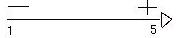
\includegraphics{images/echelle.jpg}}
\end{center}

\begin{itemize}
\item {\bf Supprimer un TD :}
	\begin{itemize}
	\item Pr{\'e}-requis : Etre identifi{\'e}.\\
	Le TD doit se trouv{\'e} dans la corbeille.
	\item Description : Il s'identifie avec son login et son mot de passe.\\
	Il affiche les fichiers contenus dans la corbeille. Il s{\'e}lectionne le TD qu'il d{\'e}sire supprimer.\\
	Il clique sur l'option {\it Suppression} et il valide sa s{\'e}lection.
	\item Post-requis : Le TD est supprimer.\\
	\end{itemize}

\item {\bf Restaurer un TD :}
	\begin{itemize}
	\item Pr{\'e}-requis : Etre identifi{\'e}.\\
	Il faut qu'au moins un TD soit dans la corbeille.
	\item Description : Il s'identifie avec son login et son mot de passe.\\
	Il affiche les fichiers contenus dans la corbeille. Il s{\'e}lectionne le TD qu'il d{\'e}sire restaurer.\\
	Il clique l'option {\it Restaurer}.\\
	Il valide sa s{\'e}lection.
	\item : Post-requis : le TD est d{\'e}plac{\'e} de la corbeille {\`a} l'emplacement qu'il occupait avant d'{\^e}tre plac{\'e} dans la corbeille.\\
	\end{itemize}
\end{itemize}


